\section{Effect of an azimuthal field}\label{result3}
In this section we use the setup of case 2 described in
\S\ref{linear}, and examine the effect of an azimuthal field so that
$B_y\neq 0$,   
parameterized by $\epsilon \equiv B_y/B_z$. However, we continute to
use $B_z$ for normalizations and $\beta$ is associated with the
vertical Alfven speed. We also extend the previous calculations to the
full disk $z\in[-Z_s,Z_s]$,  which allows us to compare the effect of
self-gravity on MRI modes with different symmetries across the
midplane. We use an isothermal disk throughout. 

\subsection{Ideal disks with MRI} 
We consider disks with $Q=0.2$ ($Q_\mathrm{2D}=~0.72$) and
$\beta=10$ in the limit of ideal MHD ($\Lambda_0=100$). Gravitational
instability is not expected because Fig. \ref{compare_growth3} shows
that even for $Q=0.18$, GI is surpressed for $\beta \lesssim 15$. 

Fig. \ref{compare_growth3_tilted} show MRI growth rates for
$B_y/B_z=0,\,1,\,2$ and $3$. We divide the modes into two catagories
depending on the extremum of magnetic energy at the midplane. 
The top panel are modes where $E_m$ has a local minimum at $z=0$ and 
the bottom panel are modes where $E_m$ has a local maximum at $z=0$. 
The latter set of modes were excluded in the previous sections by
midplane boundary conditions. 
We also plot growth rates computed in the Cowling
approximation. As expected,  $\avg{E_g}<\avg{E_m}$, so none of the
modes are energetically dominated by self-gravity. 



\begin{figure}
  \includegraphics[width=\linewidth,clip=true,trim=0cm 2cm 0cm
    0cm]{figures/compare_growth3_tilted_even.ps}  
  \includegraphics[width=\linewidth,clip=true,trim=0cm 0cm 0cm
    0.52cm]{figures/compare_growth3_tilted_odd.ps} 
  \caption{MRI growth rates in isothermal disks with $Q=~0.2$ ($Q_\mathrm{2D}=0.72$) and 
    $\beta=10$ for a range of azimuthal field strengths $B_y/B_z$. The
    dots are solutions computed from the full problem, with the
    colorbar measuring the gravitational potential perturbation, while
    the solid curves are computed from the Cowling approximation. 
    For $B_y=0$, modes in top and bottom panels have
    $W^\prime(0)=0$ and $W(0)=0$, respectively.
    \label{compare_growth3_tilted}}
\end{figure}


Consider first modes in the top panel of 
Fig. \ref{compare_growth3_tilted}. As with previous results,  
self-gravity destabilizes modes with  $k_xH\gtrsim O(1)$. Consequently, the
cut-off wavenumber is larger when SG is included. 
Destablization is most effective for purely vertical fields: with
$\epsilon=0,\, k_xH\simeq 1.4$, SG increases the growth rate by $\sim
30\%$. For $B_y=0$ we find the density perturbation $W(z)$ is an even
function. Although these modes are fundamentally magnetic, this is consistent with
\cite{goldreich65a}, who showed that SG can only destabilize 
symmetric density perturbations.  
With increasing $B_y$, we find $W$ deviates from an even
function. 
Together with the increased total magnetic pressure with 
$B_y$ (since $B_z$ is fixed), destabilization by SG weakens. 
Thus, the Cowling approximation becomes increasingly good with stronger
$B_y$ for these modes. 


The modes in the bottom panel of Fig. \ref{compare_growth3_tilted} 
display opposite behavior. For $B_y=0$ we find $W$ is odd, and
self-gravity has no effect. When $B_y>0$, $W$ deviates from an
odd function and the midplane density perturbation $|W(0)|$
increases. SG is stabilizing for these modes at all wavelengths, and
is most effective at $k_xH =  O(1)$.  
     
Fig. \ref{result_tilted} show eigenfunctions for $\epsilon=3$ and
$k_xH=1.1$ with and without the Cowling approximation.
SG significantly enhances the midplane density perturbation, making the
gravitational potential energy comparable to the magnetic energy, 
which becomes more confined near the midplane.  

\begin{figure}
  \includegraphics[width=\linewidth,clip=true,trim=0cm 1.5cm 0cm
    0cm]{figures/result_tilted_cowling.ps}  
  \includegraphics[width=\linewidth,clip=true,trim=0cm 0cm 0cm
    0.cm]{figures/result_tilted_fullsg.ps} 
  \caption{Energy densities for a MRI mode in an isothermal ideal disk
    with an azimuthal field $B_y = 3B_z$, computed in the Cowling
    approximation (top) and with full self-gravity (bottom). These
    modes correspond to those in the bottom panel of
    Fig. \ref{compare_growth3_tilted}.    
    \label{result_tilted}}
\end{figure}


To interpret the above result for modes with magnetic energy
concentrated at the midplane, we note that compressibility affects the
MRI in the presence of an azimuthal field even in a
non-self-gravitating disk. If the perturbed disk remains in vertical
hydrostatic equilibrium, then  
\begin{align} 
  |W|\sim \frac{B_y}{\mu_0\rho}|\dby|,
\end{align}
to order of magnitude in a non-SG disk. Thus a strong azimuthal field can 
cause a large density perturbation \citep{pessah05}. We checked that
for the modes in Fig. \ref{result_tilted}, vertical velocities are 
small, $|\dvz|/\left(|\dvx|^2+|\dvy|^2\right)^{1/2} \lesssim 0.2$. 

Compressibilty is enhanced by an azimuthal field, which is 
stabilizing for the MRI \citep{kim00}. %because...?
This effect is significant for $\epsilon=3$ because the azimuthal
Alfven speed is sonic.      
%maybe blaes 
Fig. \ref{result_tilted} indicates that self-gravity further enhances
compressibility, and therefore stabilization. We suspect this is
overwhelmed by the destabilization effect of SG, because the density
perturbation has an anti-symmetric component.      

\subsection{Resistive disks with GI}
Here we examine a resistive disk which permits MRI and GI by setting $Q=0.18$,
$\Lambda_0=0.1$ and $\beta=100$. 
Fig. \ref{compare_growth3_tilted_resis} show growth rates for
$\epsilon=0,\,1$ and $2$. For $B_y=0$, MRI and GI are decoupled except 
for a narrow range of $k_x$ in which the lower MRI modes transitions to
GI. Notice that the upper MRI modes intersect the GI branch. There is no
interaction because the upper MRI modes have anti-symmetric $W(z)$ whereas
the GI modes have symmetric $W(z)$. 

\begin{figure}
  \includegraphics[width=\linewidth,clip=true,trim=0cm 2cm 0cm
    0cm]{figures/compare_growth3_tilted_resis_ep0.ps}  
  \includegraphics[width=\linewidth,clip=true,trim=0cm 2cm 0cm
    0.52cm]{figures/compare_growth3_tilted_resis_ep1.ps}
  \includegraphics[width=\linewidth,clip=true,trim=0cm 0cm 0cm
    0.52cm]{figures/compare_growth3_tilted_resis_ep2.ps}
  \caption{Growth rates in isothermal resistive disks with $Q=0.18$
    ($Q_\mathrm{2D}=0.67$), $\beta=100$ and $\Lambda_0=0.1$. For
    $B_y=0$, the upper and lower MRI modes have anti-symmetric and
    symmetric density perturbations, corresponding to $W(0)=0$ and
    $W^\prime(0)=0$, respectively.  
    %anti-symmetric density
    %    perturbation $W(0) = 0$ and symmetric density perturbations,
    %    $W^\prime(0) = 0$.  
    For $B_y/B_z=2$ the
    overstable modes have non-zero real frequencies. 
    \label{compare_growth3_tilted_resis}}
\end{figure}

Introducing $B_y = B_z$ leads to an exchange in the mode
characters. For $k_xH\lesssim 0.9$ the modes on the two MRI branches
are similar to the vertical field case. However, for $k_xH\gtrsim0.9$ 
the upper MRI mode transitions to GI, for which $E_m(0)$ is a
minimum; and the lower MRI mode has $E_m(0)$ being a maximum. We find
all perturbations with  $k_xH\gtrsim0.9$ have symmetric $W(z)$. 
%small scale perts are all even 


Increasing the azimuthal field further to $B_y=2B_z$ we find
overstable MRI modes  with non-negligible real
frequencies \citep{gammie96}. An example is shown in
Fig. \ref{result_tilted_overstable}. Notice the density/potential
perturbation is off-set from the midplane. This is not possible for
pure GI \citep{goldreich65a}. Thus, these overstable MRI modes indeed
become self-gravitating, before being stabilized. 
%these may lead to significant vertical motions 

Notice also in Fig. \ref{compare_growth3_tilted_resis} the disappearence of
magnetic modes between $0.8\lesssim k_xH\lesssim 1.5$ as $B_y$ is
increased. For $B_y=2B_z$, MRI and GI are again independent, but
because they operate at distinct radial scales. This implies that
perturbations unstable to GI cannot develop MRI.       


\begin{figure}
  \includegraphics[width=\linewidth,clip=true,trim=0cm 0cm 0cm
    0cm]{figures/result_tilted_resis.ps}
  \caption{Overstable MRI mode in an isothermal resistive disk with
    $Q=0.18$ ($Q_\mathrm{2D} = 0.67$), $\Lambda_0=0.1$ and $\beta=100$. 
    The mode has a real frequency $\omega = 0.059\Omega$, or
    $\omega/\gamma \simeq 0.2 $.   
    \label{result_tilted_overstable}}
\end{figure}
